
%% bare_conf.tex
%% V1.4b
%% 2015/08/26
%% by Michael Shell
%% See:
%% http://www.michaelshell.org/
%% for current contact information.
%%
%% This is a skeleton file demonstrating the use of IEEEtran.cls
%% (requires IEEEtran.cls version 1.8b or later) with an IEEE
%% conference paper.
%%
%% Support sites:
%% http://www.michaelshell.org/tex/ieeetran/
%% http://www.ctan.org/pkg/ieeetran
%% and
%% http://www.ieee.org/

%%*************************************************************************
%% Legal Notice:
%% This code is offered as-is without any warranty either expressed or
%% implied; without even the implied warranty of MERCHANTABILITY or
%% FITNESS FOR A PARTICULAR PURPOSE! 
%% User assumes all risk.
%% In no event shall the IEEE or any contributor to this code be liable for
%% any damages or losses, including, but not limited to, incidental,
%% consequential, or any other damages, resulting from the use or misuse
%% of any information contained here.
%%
%% All comments are the opinions of their respective authors and are not
%% necessarily endorsed by the IEEE.
%%
%% This work is distributed under the LaTeX Project Public License (LPPL)
%% ( http://www.latex-project.org/ ) version 1.3, and may be freely used,
%% distributed and modified. A copy of the LPPL, version 1.3, is included
%% in the base LaTeX documentation of all distributions of LaTeX released
%% 2003/12/01 or later.
%% Retain all contribution notices and credits.
%% ** Modified files should be clearly indicated as such, including  **
%% ** renaming them and changing author support contact information. **
%%*************************************************************************


% *** Authors should verify (and, if needed, correct) their LaTeX system  ***
% *** with the testflow diagnostic prior to trusting their LaTeX platform ***
% *** with production work. The IEEE's font choices and paper sizes can   ***
% *** trigger bugs that do not appear when using other class files.       ***                          ***
% The testflow support page is at:
% http://www.michaelshell.org/tex/testflow/



\documentclass[conference]{IEEEtran}
% Some Computer Society conferences also require the compsoc mode option,
% but others use the standard conference format.
%
% If IEEEtran.cls has not been installed into the LaTeX system files,
% manually specify the path to it like:
% \documentclass[conference]{../sty/IEEEtran}





% Some very useful LaTeX packages include:
% (uncomment the ones you want to load)


% *** MISC UTILITY PACKAGES ***
%
%\usepackage{ifpdf}
% Heiko Oberdiek's ifpdf.sty is very useful if you need conditional
% compilation based on whether the output is pdf or dvi.
% usage:
% \ifpdf
%   % pdf code
% \else
%   % dvi code
% \fi
% The latest version of ifpdf.sty can be obtained from:
% http://www.ctan.org/pkg/ifpdf
% Also, note that IEEEtran.cls V1.7 and later provides a builtin
% \ifCLASSINFOpdf conditional that works the same way.
% When switching from latex to pdflatex and vice-versa, the compiler may
% have to be run twice to clear warning/error messages.






% *** CITATION PACKAGES ***
%
%\usepackage{cite}
% cite.sty was written by Donald Arseneau
% V1.6 and later of IEEEtran pre-defines the format of the cite.sty package
% \cite{} output to follow that of the IEEE. Loading the cite package will
% result in citation numbers being automatically sorted and properly
% "compressed/ranged". e.g., [1], [9], [2], [7], [5], [6] without using
% cite.sty will become [1], [2], [5]--[7], [9] using cite.sty. cite.sty's
% \cite will automatically add leading space, if needed. Use cite.sty's
% noadjust option (cite.sty V3.8 and later) if you want to turn this off
% such as if a citation ever needs to be enclosed in parenthesis.
% cite.sty is already installed on most LaTeX systems. Be sure and use
% version 5.0 (2009-03-20) and later if using hyperref.sty.
% The latest version can be obtained at:
% http://www.ctan.org/pkg/cite
% The documentation is contained in the cite.sty file itself.





\usepackage{url}
\usepackage[fleqn]{amsmath}
\usepackage{algorithm,algpseudocode}
\usepackage{mathtools}
\usepackage{gensymb}
\usepackage{csquotes}
\usepackage{placeins}
% *** GRAPHICS RELATED PACKAGES ***
%
\ifCLASSINFOpdf
  % \usepackage[pdftex]{graphicx}
  % declare the path(s) where your graphic files are
  % \graphicspath{{../pdf/}{../jpeg/}}
  % and their extensions so you won't have to specify these with
  % every instance of \includegraphics
  % \DeclareGraphicsExtensions{.pdf,.jpeg,.png}
\else
  % or other class option (dvipsone, dvipdf, if not using dvips). graphicx
  % will default to the driver specified in the system graphics.cfg if no
  % driver is specified.
  % \usepackage[dvips]{graphicx}
  % declare the path(s) where your graphic files are
  % \graphicspath{{../eps/}}
  % and their extensions so you won't have to specify these with
  % every instance of \includegraphics
  % \DeclareGraphicsExtensions{.eps}
\fi
% graphicx was written by David Carlisle and Sebastian Rahtz. It is
% required if you want graphics, photos, etc. graphicx.sty is already
% installed on most LaTeX systems. The latest version and documentation
% can be obtained at: 
% http://www.ctan.org/pkg/graphicx
% Another good source of documentation is "Using Imported Graphics in
% LaTeX2e" by Keith Reckdahl which can be found at:
% http://www.ctan.org/pkg/epslatex
%
% latex, and pdflatex in dvi mode, support graphics in encapsulated
% postscript (.eps) format. pdflatex in pdf mode supports graphics
% in .pdf, .jpeg, .png and .mps (metapost) formats. Users should ensure
% that all non-photo figures use a vector format (.eps, .pdf, .mps) and
% not a bitmapped formats (.jpeg, .png). The IEEE frowns on bitmapped formats
% which can result in "jaggedy"/blurry rendering of lines and letters as
% well as large increases in file sizes.
%
% You can find documentation about the pdfTeX application at:
% http://www.tug.org/applications/pdftex





% *** MATH PACKAGES ***
%
%\usepackage{amsmath}
% A popular package from the American Mathematical Society that provides
% many useful and powerful commands for dealing with mathematics.
%
% Note that the amsmath package sets \interdisplaylinepenalty to 10000
% thus preventing page breaks from occurring within multilines. Use:
%\interdisplaylinepenalty=2500
% after loading amsmath to restore such page breaks as IEEEtran.cls normally
% does. amsmath.sty is already installed on most LaTeX systems. The latest
% version and documentation can be obtained at:
% http://www.ctan.org/pkg/amsmath





% *** SPECIALIZED LIST PACKAGES ***
%
%\usepackage{algorithmic}
% algorithmic.sty was written by Peter Williams and Rogerio Brito.
% This package provides an algorithmic environment fo describing algorithms.
% You can use the algorithmic environment in-text or within a figure
% environment to provide for a floating algorithm. Do NOT use the algorithm
% floating environment provided by algorithm.sty (by the same authors) or
% algorithm2e.sty (by Christophe Fiorio) as the IEEE does not use dedicated
% algorithm float types and packages that provide these will not provide
% correct IEEE style captions. The latest version and documentation of
% algorithmic.sty can be obtained at:
% http://www.ctan.org/pkg/algorithms
% Also of interest may be the (relatively newer and more customizable)
% algorithmicx.sty package by Szasz Janos:
% http://www.ctan.org/pkg/algorithmicx




% *** ALIGNMENT PACKAGES ***
%
%\usepackage{array}
% Frank Mittelbach's and David Carlisle's array.sty patches and improves
% the standard LaTeX2e array and tabular environments to provide better
% appearance and additional user controls. As the default LaTeX2e table
% generation code is lacking to the point of almost being broken with
% respect to the quality of the end results, all users are strongly
% advised to use an enhanced (at the very least that provided by array.sty)
% set of table tools. array.sty is already installed on most systems. The
% latest version and documentation can be obtained at:
% http://www.ctan.org/pkg/array


% IEEEtran contains the IEEEeqnarray family of commands that can be used to
% generate multiline equations as well as matrices, tables, etc., of high
% quality.




% *** SUBFIGURE PACKAGES ***
%\ifCLASSOPTIONcompsoc
%  \usepackage[caption=false,font=normalsize,labelfont=sf,textfont=sf]{subfig}
%\else
%  \usepackage[caption=false,font=footnotesize]{subfig}
%\fi
% subfig.sty, written by Steven Douglas Cochran, is the modern replacement
% for subfigure.sty, the latter of which is no longer maintained and is
% incompatible with some LaTeX packages including fixltx2e. However,
% subfig.sty requires and automatically loads Axel Sommerfeldt's caption.sty
% which will override IEEEtran.cls' handling of captions and this will result
% in non-IEEE style figure/table captions. To prevent this problem, be sure
% and invoke subfig.sty's "caption=false" package option (available since
% subfig.sty version 1.3, 2005/06/28) as this is will preserve IEEEtran.cls
% handling of captions.
% Note that the Computer Society format requires a larger sans serif font
% than the serif footnote size font used in traditional IEEE formatting
% and thus the need to invoke different subfig.sty package options depending
% on whether compsoc mode has been enabled.
%
% The latest version and documentation of subfig.sty can be obtained at:
% http://www.ctan.org/pkg/subfig




% *** FLOAT PACKAGES ***
%
%\usepackage{fixltx2e}
% fixltx2e, the successor to the earlier fix2col.sty, was written by
% Frank Mittelbach and David Carlisle. This package corrects a few problems
% in the LaTeX2e kernel, the most notable of which is that in current
% LaTeX2e releases, the ordering of single and double column floats is not
% guaranteed to be preserved. Thus, an unpatched LaTeX2e can allow a
% single column figure to be placed prior to an earlier double column
% figure.
% Be aware that LaTeX2e kernels dated 2015 and later have fixltx2e.sty's
% corrections already built into the system in which case a warning will
% be issued if an attempt is made to load fixltx2e.sty as it is no longer
% needed.
% The latest version and documentation can be found at:
% http://www.ctan.org/pkg/fixltx2e


%\usepackage{stfloats}
% stfloats.sty was written by Sigitas Tolusis. This package gives LaTeX2e
% the ability to do double column floats at the bottom of the page as well
% as the top. (e.g., "\begin{figure*}[!b]" is not normally possible in
% LaTeX2e). It also provides a command:
%\fnbelowfloat
% to enable the placement of footnotes below bottom floats (the standard
% LaTeX2e kernel puts them above bottom floats). This is an invasive package
% which rewrites many portions of the LaTeX2e float routines. It may not work
% with other packages that modify the LaTeX2e float routines. The latest
% version and documentation can be obtained at:
% http://www.ctan.org/pkg/stfloats
% Do not use the stfloats baselinefloat ability as the IEEE does not allow
% \baselineskip to stretch. Authors submitting work to the IEEE should note
% that the IEEE rarely uses double column equations and that authors should try
% to avoid such use. Do not be tempted to use the cuted.sty or midfloat.sty
% packages (also by Sigitas Tolusis) as the IEEE does not format its papers in
% such ways.
% Do not attempt to use stfloats with fixltx2e as they are incompatible.
% Instead, use Morten Hogholm'a dblfloatfix which combines the features
% of both fixltx2e and stfloats:
%
% \usepackage{dblfloatfix}
% The latest version can be found at:
% http://www.ctan.org/pkg/dblfloatfix




% *** PDF, URL AND HYPERLINK PACKAGES ***
%
%\usepackage{url}
% url.sty was written by Donald Arseneau. It provides better support for
% handling and breaking URLs. url.sty is already installed on most LaTeX
% systems. The latest version and documentation can be obtained at:
% http://www.ctan.org/pkg/url
% Basically, \url{my_url_here}.




% *** Do not adjust lengths that control margins, column widths, etc. ***
% *** Do not use packages that alter fonts (such as pslatex).         ***
% There should be no need to do such things with IEEEtran.cls V1.6 and later.
% (Unless specifically asked to do so by the journal or conference you plan
% to submit to, of course. )


% correct bad hyphenation here
\hyphenation{op-tical net-works semi-conduc-tor}


\begin{document}
%
% paper title
% Titles are generally capitalized except for words such as a, an, and, as,
% at, but, by, for, in, nor, of, on, or, the, to and up, which are usually
% not capitalized unless they are the first or last word of the title.
% Linebreaks \\ can be used within to get better formatting as desired.
% Do not put math or special symbols in the title.
\title{Human Family Tree\\Mitochondrial Eve}


% author names and affiliations
% use a multiple column layout for up to three different
% affiliations
\author{\IEEEauthorblockN{Gopal Menon}
\IEEEauthorblockA{Computer Science Department\\
Utah State University\\
Logan, Utah 84322\\
Email: gopal.menon@aggiemail.usu.edu}
}

% conference papers do not typically use \thanks and this command
% is locked out in conference mode. If really needed, such as for
% the acknowledgment of grants, issue a \IEEEoverridecommandlockouts
% after \documentclass

% for over three affiliations, or if they all won't fit within the width
% of the page, use this alternative format:
% 
%\author{\IEEEauthorblockN{Michael Shell\IEEEauthorrefmark{1},
%Homer Simpson\IEEEauthorrefmark{2},
%James Kirk\IEEEauthorrefmark{3}, 
%Montgomery Scott\IEEEauthorrefmark{3} and
%Eldon Tyrell\IEEEauthorrefmark{4}}
%\IEEEauthorblockA{\IEEEauthorrefmark{1}School of Electrical and Computer Engineering\\
%Georgia Institute of Technology,
%Atlanta, Georgia 30332--0250\\ Email: see http://www.michaelshell.org/contact.html}
%\IEEEauthorblockA{\IEEEauthorrefmark{2}Twentieth Century Fox, Springfield, USA\\
%Email: homer@thesimpsons.com}
%\IEEEauthorblockA{\IEEEauthorrefmark{3}Starfleet Academy, San Francisco, California 96678-2391\\
%Telephone: (800) 555--1212, Fax: (888) 555--1212}
%\IEEEauthorblockA{\IEEEauthorrefmark{4}Tyrell Inc., 123 Replicant Street, Los Angeles, California 90210--4321}}




% use for special paper notices
%\IEEEspecialpapernotice{(Invited Paper)}




% make the title area
\maketitle

% As a general rule, do not put math, special symbols or citations
% in the abstract
\begin{abstract}
Cann, Stoneking and Wilson as described in their paper \cite{mtDnaPaper} on Mitochondrial DNA and human evolution used 147 human mitochondrial DNA (mtDNA) samples, and performed restriction mapping on each sample. The restriction sites were mapped using known human mtDNA sequences. The number of restriction site differences between each pair of individuals gave them the extent of the nucleotide sequence divergence. mtDNA is inherited from the mother and unlike nuclear DNA, does not go through combination of DNA from both the parents. All living human beings are thought to have descended from one common ancestor \cite{wikiMtEve}. This is not to be thought of as a specific person, since whenever an ancient mtDNA branch dies out, the most recent common ancestor (MRCA) moves to a more recent female ancestor. The restriction site differences between all the pairs of individuals were used to induce a genealogical tree shown in figure \ref{HumanTree}. This tree suggested that human beings originated in Africa and then settled the rest of the planet as shown in figure \ref{HumanMigration}. The aim of the project is to start with mtDNA samples from a varied group of people and compute the alignment distance matrix for all pairs of samples. Using this matrix, an evolutionary tree and hierarchical clustering algorithm needs to be implemented in order to induce a tree similar to the one shown in figure \ref{HumanTree}. 
\end{abstract}

\begin{figure}[!t]
\centering
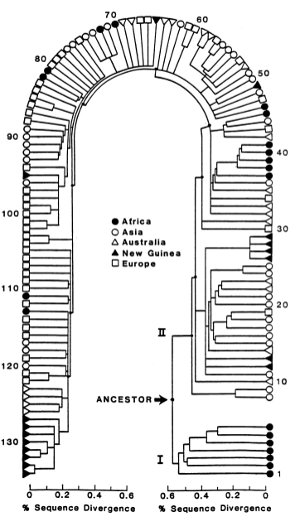
\includegraphics[width=3.5in]{./figures/eve.jpg}
\caption{Human geneological tree based on mtDNA samples \cite{mtDnaPaper}}
\label{HumanTree}
\end{figure}

\begin{figure}[!t]
\centering
\includegraphics[width=3.5in]{./figures/mtDNA.png}
\caption{Mitochondrial DNA\cite{KhanAcademy}}
\label{mtDNA}
\end{figure}

\begin{figure}[!t]
\centering
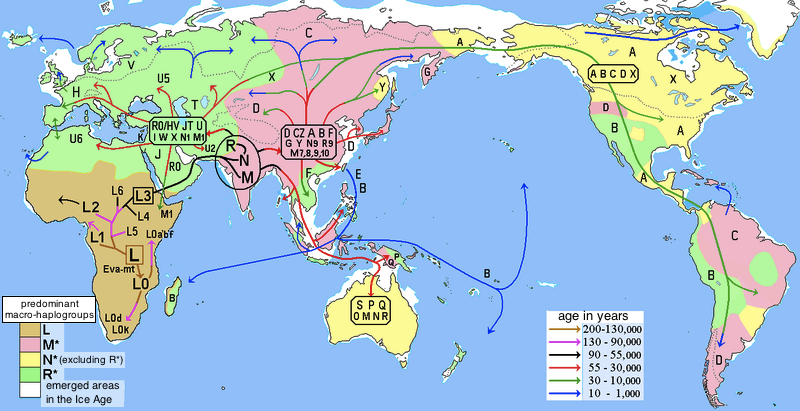
\includegraphics[width=3.5in]{./figures/Human_migrations_and_mitochondrial_haplogroups.png}
\caption{Human migrations and mitochondrial haplogroups. The letters stand for haplogroups, which are groups of people who share a common ancestor \cite{Haplogroup}.}
\label{HumanMigration}
\end{figure}
% no keywords




% For peer review papers, you can put extra information on the cover
% page as needed:
% \ifCLASSOPTIONpeerreview
% \begin{center} \bfseries EDICS Category: 3-BBND \end{center}
% \fi
%
% For peerreview papers, this IEEEtran command inserts a page break and
% creates the second title. It will be ignored for other modes.
\IEEEpeerreviewmaketitle

\section{Biological problem and its significance}
mtDNA is comprised of 16,569 base pairs and is present only in cells in the animal kingdom. Figure \ref{mtDNA} shows a graphic of mtDNA within a cell. It is contained in almost every cell of the body and is inherited only from the mother. In this regard, it is different from nuclear DNA that consists of genetic material from both parents. mtDNA is thought to be a bacterium like organism that had been captured by a cell. It does not have the ability for error checking during replication and is more susceptible to mutations than nuclear DNA. Restriction site differences or the edit distance between two samples can be used as an estimate on how many years ago was the common ancestor alive. Individuals with low edit distances between their mtDNA will have a more recent common ancestor. When humans migrate to a particular region, after a period of time, that region will have many humans with one of the migrated human females as a common ancestor. This common ancestor will be be more recent than the common ancestor for a descendant of one of the migrated humans and a descendant from the original population that did not migrate. mtDNA edit distance can be thus used to induce genealogical trees of the form shown in figure \ref{HumanTree}. This can lead to an understanding of the origins of populations of certain geographic regions and human migration paths. The paper written by Cann et. al. suggests that human beings originated in Africa since the common ancestor shown in figure \ref{HumanTree} would need to be African in order to minimize the number of intercontinental migrations needed to account for the geographic distribution of mtDNA types.\\

The human mtDNA molecular clock is the rate at which mutations have been accumulating in the mitochondrial genome. The mutation rate differs between coding and non-coding regions of the mtDNA. Coding region mutations may be fatal or may lead to other complications and due to this reason, mutations in this region will lead to purifying selections. Some studies avoid coding region mutations, while other studies consider both regions 
 and apply a correction factor for selection in coding region. 

\FloatBarrier
\section{Other Similar studies}

\subsection{Neanderthal DNA Sequences and Origin of Modern Humans}

As part of the study \cite{Neanderthals}, DNA material was extracted from a Neanderthal specimen found in 1856 in western Germany. A hitherto unknown mitochondrial mtDNA sequence was found in the specimen. Sequence comparisons with human mtDNA sequences, as well as phylogenetic analyses, showed that the Neanderthal sequence fell outside the variation of modern humans. Furthermore, the age of the common ancestor of the Neanderthal and modern human mtDNAs was estimated to be four times greater than that of the common ancestor of human mtDNAs. This suggested that Neanderthals went extinct without contributing mtDNA to modern humans as an ancestor.

\subsection{An early modern human from Romania with a recent Neanderthal ancestor}

Neanderthals are thought to have disappeared in Europe ~39,000-41,000 years ago but they have contributed one to three percent of the DNA of present-day people in Eurasia. In the study \cite{Romania}, they analyzed DNA from a 37,000-42,000-year-old modern human from Pestera cu Oase, Romania. Although the specimen contained small amounts of human DNA, they used an enrichment strategy to isolate sites that were informative about its relationship to Neanderthals and present-day humans. They found that on the order of six to nine percent of the genome of the Oase individual was derived from Neanderthals, more than any other modern human sequenced to date. Three chromosomal segments of Neanderthal ancestry were over 50 centimorgans in size, indicating that this individual had a Neanderthal ancestor as recently as four to six generations back. However, the Oase individual did not share more alleles with later Europeans than with East Asians, suggesting that the Oase population did not contribute substantially to later humans in Europe.

\FloatBarrier
\section{Computer science problem}
\subsection{Edit Distance}
The edit distance between two mtDNA sequences can be found using Dynamic Programming. Since only the edit distance score is needed, the computation can be done using an array of two columns with the number of rows equal to the length of a mtDNA sequence. For 2699 samples (see figure \ref{DataSize}), 3.6 million edit distance computations would need to be done. Even with C++, this amount of computation would take too long to execute. In order to complete the project, a subset of the samples was used. A penalty of $1$ was used for insertion, deletion and substitution during edit distance computation.

\FloatBarrier
\subsection{Clustering}
The evolutionary tree was found out by running clustering on the mtDNA samples using the edit distance as the input to clustering. mtDNA samples with smaller edit distances would form clusters. These would be clusters corresponding to leaves of the evolutionary tree with a common ancestor. The clusters would then be combined based on the distance between the cluster centroids. This would give us common ancestors of the initial clusters. The process would be repeated till we find a common ancestor for all the mtDNA samples. 

The Unweighted Pair Group Method with Arithmetic Mean (UPGMA) algorithm \cite{TextBook1} was used for heirarchical clustering of mtDNA samples. The length of an edge between two clusters will be the difference in heights between them and will be a measure of their separation in years. Given two clusters $C_1$ and $C_2$, the UPGMA algorithm defines the distance between them to be the average pairwise distance: \\

$D(C_1, C_2) =\frac{1}{\left | C_1 \right | \left | C_2 \right |} \sum_{i \epsilon C_1} \sum_{j \epsilon C_2} D\left (i, j \right )$\\

Algorithm \ref{UPGMAAlgorithm} shows the details of the algorithm and it is called with parameters $D$, the edit distance matrix and $n$ the number of elements.
\floatevery{algorithm}{\setlength\hsize{7cm}}
\begin{minipage}{\linewidth}
  \begin{algorithm}[H]
    \caption{UPGMA Algorithm}\label{UPGMAAlgorithm}
    \begin{algorithmic}[1]
      \Procedure{UPGMAAlgorithm.$UPGMA(D, n)$}{}
        \State Form $n$ clusters, each with a single element
        \State \parbox[t]{\dimexpr\linewidth-\algorithmicindent}{Construct graph $T$ by assigning isolated vertex to each cluster\strut}
        \State Assign height $h(v) = 0$ to every vertex $v$ in graph
        \While{there is more than one cluster}
          \State Find two closest clusters $C_1$ and $C_2$
          \State \parbox[t]{\dimexpr\linewidth-\algorithmicindent}{Merge $C_1$ and $C_2$ into a new cluster $C$ with $\left | C_1 \right | + \left | C_2 \right  |$ elements\strut}
          \For{every cluster $C^* \not = C$}
            \State \parbox[t]{\dimexpr\linewidth-\algorithmicindent}{$D(C, C^*) =\frac{1}{\left | C \right | \left | C^* \right |} \sum_{i \epsilon C} \sum_{j \epsilon C^*} D\left (i, j \right )$\strut}
          \EndFor
          \State  \parbox[t]{\dimexpr\linewidth-\algorithmicindent}{Add a new vertex $C$ to $T$ and connect to vertices $C_1$ and $C_2$\strut}
          \State Vertex height $h(C) = \frac{D(C_1, C_2)}{2}$
          \State Assign length $h(C) - h(C_1)$ to the edge $(C_1, C)$
          \State Assign length $h(C) - h(C_2)$ to the edge $(C_2, C)$
          \State \parbox[t]{\dimexpr\linewidth-\algorithmicindent}{Remove rows and columns of $D$ corresponding to $C_1$ and $C_2$\strut}
          \State \parbox[t]{\dimexpr\linewidth-\algorithmicindent}{Add a row and column to $D$ for the new cluster $C$\strut}
        \EndWhile
       \State return $T$
      \EndProcedure
    \end{algorithmic}
  \end{algorithm}
\end{minipage}\\\\

\begin{figure}[!t]
\centering
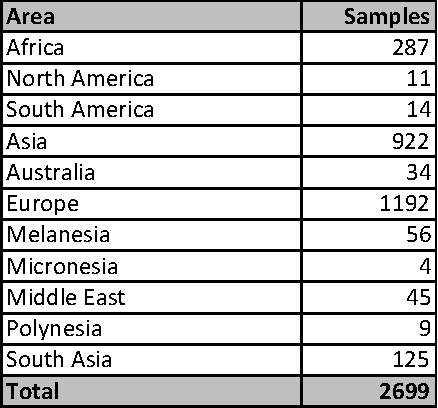
\includegraphics[width=2.5in]{./figures/DataSize.pdf}
\caption{Number of mtDNA samples from each geographic regions}
\label{DataSize}
\end{figure}

\section{Tasks}

\subsection{Download mtDNA sequences}
A subset of the 2699 mtDNA sequences was downloaded into text files from the Human Mitochondrial Genome Database \cite{mtDnaDatabase}. Furthermore, clustering was run on a further subset. The subset details can be seen by referring to the phylogenetic trees in this report.

\subsection{Compute Edit Distance Matrix}

The edit distance matrix for the subset of the samples was computed by finding out the edit distance for all possible pairs of mtDNA. 

\subsection{Clustering and Evolutionary Tree}
Clustering was done using the UPGMA (Unweighted Pair Group Method with Arithmetic Mean) clustering algorithm as described above in order to create an evolutionary tree.

\subsection{Evolutionary Tree Illustration}
A script for showing the evolutionary tree was generated during clustering. The script was generated in the Newick format \cite{Newick}. An example of this format is shown in figure \ref{NewickFormat}. Nested parentheses are used for specifying heirarchy where node name is followed by colon and node height. The Newick format script for the tree shown in figure \ref{NewickFormat} is $(A:0.1,B:0.2,(C:0.3,D:0.4):0.5)$.


\begin{figure}[!t]
\centering
\includegraphics[width=3.5in]{./figures/Newick.png}
\caption{Newick format illustration \cite{Newick} .}
\label{NewickFormat}
\end{figure}

\FloatBarrier
\section{Results}

\FloatBarrier
\subsection{Africa Evolutionary Tree}

The tree is shown in figure \ref{AfricaTree}. The number $9.99$ at the bottom left of the tree is the scale and represents the edit distance. We can see that groups with large separation (with a less recent common ancestor) are all from sub-saharan Africa. They appear to be the humans whose common ancestor is Mitochondrial Eve. People who live near to each other appear to have a more recent common ancestor like in the case of Morocco and Canary Islands

\begin{figure}[!t]
\centering
\includegraphics[width=3.5in]{./figures/AfricaTree.png}
\caption{Africa Phylogenetic Tree}
\label{AfricaTree}
\end{figure}

\FloatBarrier
\subsection{South Asia and Middle East Evolutionary Tree}

The tree is shown in figure \ref{SouthAsianMiddleEastTree}. Mainland Indians (figure \ref{KalPenn}) are closer to Onges (figure \ref{OngeWoman}) than they are to Iraqis (figure \ref{Maliki}). Outward features are thought to be  a more recent development from around 50,000 years ago \cite{TextBook1} and these cannot be used a guide to gauge the closeness of relations between peoples.

\begin{figure}[!t]
\centering
\includegraphics[width=3.5in]{./figures/SouthAsianMiddleEastTree.png}
\caption{South Asia and Middle East Phylogenetic Tree}
\label{SouthAsianMiddleEastTree}
\end{figure}

\begin{figure}[!t]
\centering
\includegraphics[width=3.5in]{./figures/CalPenn.png}
\caption{Kal Penn - Actor of Gujrati Indian ethnicity}
\label{KalPenn}
\end{figure}

\begin{figure}[!t]
\centering
\includegraphics[width=2.0in]{./figures/OngeWoman.png}
\caption{Woman of Onge Indian ethnicity}
\label{OngeWoman}
\end{figure}

\begin{figure}[!t]
\centering
\includegraphics[width=2.0in]{./figures/Maliki.png}
\caption{Nouri Al-Maliki - ex Prime Minister of Iraq}
\label{Maliki}
\end{figure}

\FloatBarrier
\subsection{Asia Evolutionary Tree}

The tree is shown in figure \ref{AsianTree}. Japanese and Han Chinese are very closely related. However their culture and customs are very different. Khirgiz and Korean mtDNA samples were identical and this is the reason these two sample show a very recent common ancestor. This was a problem with the data.

\begin{figure}[!t]
\centering
\includegraphics[width=3.5in]{./figures/AsianTree.png}
\caption{Asia Phylogenetic Tree}
\label{AsianTree}
\end{figure}

\FloatBarrier
\subsection{Europe Evolutionary Tree}

The tree is shown in figure \ref{EuropeTree}. People from Spain are not very close in terms of a recent common ancestor. This can be seen in Spanish samples from Andalusia, Leon, Galicia and Maragato. Similar is the case with Italians. French people are closer to Crimean Tatars than to Europeans from closer regions.The European American seems to have a matrilineal ancestor from Southern Italy.


\begin{figure}[!t]
\centering
\includegraphics[width=3.5in]{./figures/EuropeTree.png}
\caption{Europe Phylogenetic Tree}
\label{EuropeTree}
\end{figure}

\FloatBarrier
\subsection{Oceania and Pacific Islands Evolutionary Tree}

The tree is shown in figure \ref{IslandsTree}. Papua New Guinea (PNG) people seem to be further apart from each other than other groups in the tree with a common ancestor.
PNG is on the eastern side of one island and is not a very large country.

\begin{figure}[!t]
\centering
\includegraphics[width=3.5in]{./figures/IslandsTree.png}
\caption{Oceania and Pacific Islands Evolutionary Tree}
\label{IslandsTree}
\end{figure}

\FloatBarrier
\subsection{North and South America Evolutionary Tree}

The tree shown in figure \ref{AmericasTree}. North American and Guarini (from different continents) samples are closer than North American and Navajo (from the same continent).

\begin{figure}[!t]
\centering
\includegraphics[width=3.5in]{./figures/AmericasTree.png}
\caption{North and South America Phylogenetic Tree}
\label{AmericasTree}
\end{figure}

\FloatBarrier
\subsection{World Evolutionary Tree}

The tree is shown in figure \ref{AbridgedWorldTree}. People are mostly grouped by geographic region. Some unexplained cases are Guarini (from South America) and Navajo (from North America) are in separate branches altogether. I would have expected them to be closer. Nicobarese (from Indian islands) and Piman (from North America) have a comparatively recent common ancestor even they are on different continents.

\begin{figure}[!t]
\centering
\includegraphics[width=3.5in]{./figures/AbridgedWorldTree.png}
\caption{World Phylogenetic Tree}
\label{AbridgedWorldTree}
\end{figure}

\FloatBarrier
\section{Summary and Conclusions}
From the phylogenetic trees that were created, we can see that humans from a particular geographic region usually have a more recent common ancestor. However there are cases where mtDNA samples from regions that were far apart, were seen to be closer than the ones where the regions were closer. I am not sure why this is the case. But it is possible that in these cases, the individual had a mixed ancestry and/or lost the details on their matrilineal lineage. In places like Papua New Guinea and Spain, we can see that within a small geographic region, there is a large separation between the samples and their common ancestor. This is possibly due to geographic isolation that prevented the people from interacting with people from other regions. As we saw in the case of the mainland Indians, Onges and Iraqis, outward features for people closer in terms of a recent common ancestor, may be very different. Outward features for people with a more ancient common ancestor may be more similar. \\

The world family tree in figure \ref{AbridgedWorldTree} did not help me in constructing a human migration as shown in figure \ref{HumanMigration}. 


\FloatBarrier
\begin{thebibliography}{1}

\bibitem{KhanAcademy}
\enquote{Khan Academy.} \textit{Khan Academy}. N.p., n.d. Web. 10 Aug. 2016.

\bibitem{mtDnaPaper}
Cann, L. C., M. Stoneking, and A. C. Wilson. \enquote{Mitochondrial DNA and human evolution.} \textit{Nature} 325 (1987): 1-5.

\bibitem{wikiMtEve}
\enquote{Mitochondrial Eve.} \textit{Wikipedia}. Wikimedia Foundation, n.d. Web. 24 July 2016.

\bibitem{mtDnaDatabase}
Ingman, M. \& Gyllensten, U. mtDB: Human Mitochondrial Genome Database, a resource for population genetics and medical sciences. Nucleic Acids Res 34, D749-D751 (2006).

\bibitem{TextBook1}
Jones, Neil C., and Pavel Pevzner. \textit{An Introduction to Bioinformatics Algorithms.} Cambridge, MA: MIT, 2004. Print.

\bibitem{Haplogroup}
\enquote{Human Mitochondrial DNA Haplogroup.} \textit{Wikipedia}. Wikimedia Foundation, n.d. Web. 25 July 2016.
\bibitem{Newick} 
\enquote{Newick Format.} \textit{Wikipedia}. Wikimedia Foundation, n.d. Web. 08 Aug. 2016.
\bibitem{Neanderthals}
Krings, Matthias, et al. \enquote{Neandertal DNA sequences and the origin of modern humans.} cell 90.1 (1997): 19-30.

\bibitem{Romania}
Fu, Qiaomei, et al. \enquote{An early modern human from Romania with a recent Neanderthal ancestor.} \textit{Nature} 524.7564 (2015): 216-219.
\end{thebibliography}

\section{Appendix}
\subsection{Running the program}
\label{sssec:num1} 

The program runs clustering on the mtDNA samples that are listed in the text file \textit{fileListing.txt}. This text file must contain the names of the downloaded mtDNA sample files that are in text format. The mtDNA samples should have nucleotide strings without embedded spaces. They can be separated by line feeds. The input data should be in the format that the human mtDNA samples are in the mtDNA database \cite{mtDnaDatabase}.

\subsection{Obtaining the tree script}
The program will create the script in file \textit{WorldTreeScript.txt}. This file can be uploaded to the website \url{http://etetoolkit.org/treeview/} for viewing the tree.

\end{document}
